\chapter{Algorithm Description}\label{ch:algorithm}

The algorithm described in this chapter and its preliminary test
result on real flight data was published in
\cite{zhang_obstacle_2012}. The program was implemented in Python
programming language \cite{_python_????}. An open source machine
vision library OpenCV was utilized to perform feature extraction and
tracking. The feature extraction method used was the Shi-Tomasi corner
detector \cite{shi_good_1994}. Feature tracking was accomplished
through the pyramid implementation of Lucas-Kanade optical flow method
\cite{bouguet_pyramidal_1999}. Both algorithms were implemented in
OpenCV. 

\section{Camera Centric Inverse Depth Parameterization}
Figure \ref{fig:algo1} shows the parameters definition in inverse
depth parameterization.

\begin{figure}[h]
\centering
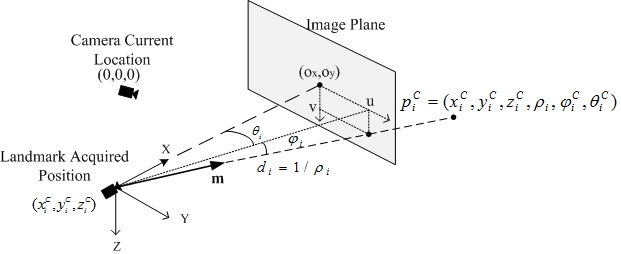
\includegraphics[width=10cm, keepaspectratio=true]{./Figures/idp.jpg}
\caption{Inverse Depth Parameterization}
\label{fig:algo1}
\end{figure}

A 3D scene point $p_{i}^{C}$ can be defined by 6 parameters with the 
superscript $C$ representing a camera reference frame and $i$
representing the feature number:
\begin{equation}
p_{i}^{C}=\begin{bmatrix}
x_{i}^{C} & y_{i}^{C} & z_{i}^{C} & \rho _{i} & \varphi _{i}^{C} & 
\theta _{i}^{C} 
\end{bmatrix}
\end{equation}
The first three parameters $[x_{i}^{C}, y_{i}^{C}, z_{i}^{C}]$
represent the initial position where the feature is first observed.
$\rho_{i} = 1/d_i$ is the inverse distance from the initialization position
to the feature. The elevation-azimuth pair $[\varphi_{i}^{C},
\theta_{i}^{C}]$ encodes a unit vector pointing from the
initialization point to the feature. The vector is given by
\begin{equation}
\label{eq:m}
m(\phi_{i}^{C}, \theta_{i}^{C})=\begin{bmatrix}
\cos\varphi_{i}^{C}\cos\theta _{i}^{C} \\
\cos\varphi_{i}^{C}\sin\theta _{i}^{C} \\
\sin\varphi_{i}^{C}
\end{bmatrix}
\end{equation}

\noindent Given the a vector $[h_x, h_y, h_z]$, one can also find the
elevation-azimuth angles $[\varphi, \theta]$ by

\begin{equation}
\label{eq:m_inv_varphi}
\varphi 
=arctan\left(\frac{h_{z}}{\sqrt{h_x^2+h_y^2}}\right)
\end{equation}

\begin{equation}
\label{eq:m_inv_theta}
\theta =arctan\left(\frac{h_{y}}{h_{x}}\right)
\end{equation}


\section{Modeling the System with Extended Kalman 
Filter}

\subsection{Full State Vector}

The EKF full state vector is defined as 

\begin{equation}
x=\begin{bmatrix}
OX_{W}^{C} & c^{C} & r^{C} & p_{1}^{C} & p_{2}^{C} & \ldots 
\end{bmatrix}^T
\end{equation}

\noindent where $OX_{W}^{C}= \begin{bmatrix}O_{x}^{C} & O_{y}^{C} &
  O_{z}^{C} & W_{x}^{C} & W_{y}^{C} & W_{z}^{C} \end{bmatrix}^{T}$
contains translation parameters $O_{x,y,z}^{C}$ and rotation
parameters $W_{x,y,z}^{C}$ that represents the world frame position
and orientation referenced to the camera frame.
$\left(c^{C},r^{C}\right)^{T}$ represents the camera translation and
rotation motion frame by frame, and $p_{i}^{C}$ contains the feature
parameters as described in the previous section.

\subsection{Prediction}

For a prediction step at time $k$, the world frame parameter $OX_W^C$
and features parameters $p_i^C$ are kept unchanged from time $k-1$.
The camera parameters are updated using the new inertial measurements:
velocity $v^{C}$, acceleration $a^{C}$, and rate of change $w^{C}$ in
roll, pitch, and azimuth. The camera motion parameters at time $k$ are
then
\begin{multline}
\begin{bmatrix}
OX_{W}^{C} & c^{C} & r^{C} & p_{1}^{C}& p_{2}^{C} & \vdots & p_n^C
\end{bmatrix}_{k}^T \\
=\begin{bmatrix}
OX_{W,k-1}^{C} & c_{measured}^{C} & r_{measured}^{C} & p_{1,k-1}^{C} &
p_{2,k-1}^{C} & \vdots & p_{n,k-1}^C
\end{bmatrix}^T
\end{multline}

\noindent where 

$$c_{measured}^{C}=v_{measured}^{C}\Delta t+ \frac{1}{2}a_{measured}^{C}\Delta t^{2}$$
$$r_{measured}^{C}=r_{k-1}^{C}+ w_{measured}^{C}$$

\noindent and $\Delta t$ is the time elapsed from frame to frame. 

\subsection{Measurement Model}

Each observed feature is related to the camera motion through the
measurement model (figure \ref{fig:measurement_model}). This
relationship enables a correction on the camera motion and features
parameters based on the features locations observed in the image.

\begin{figure}[h]
\centering
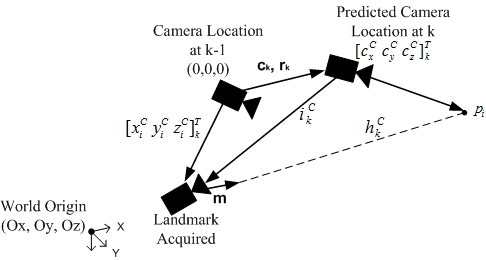
\includegraphics[width=10cm, keepaspectratio=true]{./Figures/measurement_model.jpg}
\caption{Measurement Model}
\label{fig:measurement_model}
\end{figure}

For a feature $p_{i}^{C}$, the vector $h^{R}$ pointing from the 
predicted camera location to the feature initialization position is 

\begin{equation}
h_{k}^{R}=\begin{bmatrix}
x_{i}^{C} \\
y_{i}^{C} \\
z_{i}^{C} \\
\end{bmatrix}_{k}-\begin{bmatrix}
c_{x}^{C} \\
c_{y}^{C} \\
c_{z}^{C} \\
\end{bmatrix}_{k}
\end{equation}

The normalized vector pointing from the predicted camera position to the 
feature at time k is then 

\begin{equation}
  h_{k}^{C}=Q^{-1}\left(r_{k}^{C}\right)\left(\rho _{k}h_{k}^{R}+m\left(\varphi_{ 
        k}^{C},\theta _{k}^{C}\right)\right)
\end{equation}

\noindent where $Q^{-1}(r_{k}^{C})$ is the inverse rotation matrix from the 
camera frame at time $k-1$ to camera frame at time $k$. From vector 
$h_{k}^{C}$, the feature location on image plane can be found by

\begin{equation}
h_{k}^{U}= \begin{bmatrix}
u_{k} \\
v_{k} \\
\end{bmatrix}=\begin{bmatrix}
\frac{f_{x}h_{y,k}^{C}}{h_{x,k}^{C}} \\
\frac{f_{y}h_{z,k}^{C}}{h_{x,k}^{C}} \\
\end{bmatrix}
\end{equation}

\noindent where $f_{x}$ and $f_{y}$ is the scaling factor of the projection 
obtained through camera calibration.

Since the measurement model is non-linear, the equation must be
linearized to calculate the Kalman gain $K$. Detail formulation for
linearization is given in appendix \ref{ch:appendix3}.

\subsection{Composition Step}

The correction using measurement model described above still has all
its parameters defined in camera frame at step $k-1$. Therefore, a
coordinate transformation must be done to transform all parameters,
and error matrix into camera frame at step k so that the next cycle of
tracking can be continued. World reference frame parameters from step
$k-1$ to step $k$ is related by

\begin{equation}
\begin{bmatrix}
O_{x}^{C_{k}} \\
O_{y}^{C_k} \\
O_{z}^{C_k} \\
\end{bmatrix}_{k}=Q^{-1}(r_{k}^{C_{k-1}})\left(
\begin{bmatrix}
O_{x}^{C_{k-1}} \\
O_{y}^{C_{k-1}} \\
O_{z}^{C_{k-1}} \\
\end{bmatrix}_{k}- \begin{bmatrix}
c_{x}^{C_{k-1}} \\
c_{y}^{C_{k-1}} \\
c_{z}^{C_{k-1}} \\
\end{bmatrix}_{k}\right)
\end{equation}

\begin{equation}
\begin{bmatrix}
W_{x}^{C_{k}} \\
W_{y}^{C_{k}} \\
W_{z}^{C_{k}} \\
\end{bmatrix}_{k-1}= \begin{bmatrix}
W_{x}^{C_{k-1}} \\
W_{y}^{C_{k-1}} \\
W_{z}^{C_{k-1}} \\
\end{bmatrix}_{k}-r^{C_{k-1}}
\end{equation}

Feature parameters in the new camera frame are related to the previous frame 
by

\begin{equation}
\begin{bmatrix}
x_{i}^{C_{k}} \\
y_{i}^{C_{k}} \\
z_{i}^{C_{k}} \\
\end{bmatrix}_{k}=Q^{-1}(r^{C_{k-1}})\left(
\begin{bmatrix}
x_{i}^{C_{k-1}} \\
y_{i}^{C_{k-1}} \\
z_{i}^{C_{k-1}} \\
\end{bmatrix}_{k}- \begin{bmatrix}
c_{x}^{C_{k-1}} \\
c_{y}^{C_{k-1}} \\
c_{z}^{C_{k-1}} \\
\end{bmatrix}_{k}\right)
\end{equation}

\begin{equation}
\begin{bmatrix}
\rho_{i} \\
\varphi_{i}^{C_{k}} \\
\theta_{i}^{C_{k}} \\
\end{bmatrix}_{k}=
\begin{bmatrix}
\rho _{i} \\
m^{-1}\left(Q^{-1}(r^{C_{k-1}})m(\varphi _{i, k}^{C_{k-1}}, \theta _{i, k}^{C_{k-1}})\right) \\
\end{bmatrix}
\end{equation}

\noindent where $\rho_i$ is a scaler, and doesn't need transformation.
$m(\varphi_{i, k}^{C_{k-1}}, \theta_{i, k}^{C_{k-1}})$ is the unit
vector pointing from the initialization point to the feature seen by
the camera at step $k-1$. $m^{-1}$ represent the operator that convert
the unit vector back to $[\varphi, \theta]$ angles as defined in
equation (\ref{eq:m_inv_varphi}) (\ref{eq:m_inv_theta}).

The covariance matrix is also affected by this transformation. The new
covariance matrix is related to the old one by

\begin{equation}
P_{k}^{C_{k}}=J_{C_{k-1}\to C_{k}}P_{k}^{C_{k-1}}J_{C_{k-1}\to C_{k}}^{T}
\end{equation}

\noindent where $J_{C_{k-1} \to C_k}$ is the Jacobian matrix of the
composition equations. Detail derivation of the Jacobian matrix is
given in appendix D \ref{?}  

\subsection{Filter Initialization}
\subsubsection{Initialize the State Vector}

State vectors are initialized at the first frame. The world origin 
coordinate and orientation, camera motions, and the feature reference 
points are all initialized to zeros, with variance equals to the 
smallest machine number. 

\begin{equation}
\label{eq:OX_init}
OX_{W}^{C}=\begin{bmatrix}0&0&0&0&0&0\end{bmatrix}^T 
\end{equation}

\begin{equation}
c^{C}=\begin{bmatrix}0&0&0\end{bmatrix}^T
\end{equation}

\begin{equation}
r^{C}=\begin{bmatrix}0&0&0\end{bmatrix}^T
\end{equation}

\begin{equation}
p_{i}^{C}=\begin{bmatrix}0&0&0&\rho _{i}&\varphi_{i}^C&\theta_{i}^C\end{bmatrix}^T
\end{equation}

The inverse distance $\rho$ of all features are initialized to 0.1
($d=100m$). The features elevation-azimuth pair $[\varphi _{i}^{C},
\theta _{i}^{C}]$ is extracted from features coordinates in image
plane. First, a vector pointing from camera optical center to feature
can be defined by

\begin{equation}
\label{eq:init_feature_unit_vec}
h^{C}=\begin{bmatrix}
h_{x}^{C}\\
h_{y}^{C}\\
h_{z}^{C}\\
\end{bmatrix}
 = \begin{bmatrix}
1 \\
(u-c_x) \cdot f_{x} \\
(v-c_y) \cdot f_{y} \\
\end{bmatrix}
\end{equation}

\noindent where $[u, v]$ is the feature coordinate in the image, $
[f_{x}, f_{y}]$ is the scaling factor of the projection from the scene
to image plane, $[c_x, c_y]$ is the coordinate where the optical axis
intersects the image plane. The elevation-azimuth pair $[\varphi
_{i}^{C}, \theta _{i}^{C}]$ can then be directly calculated from
$h^{C}$ using equation (\ref{eq:m_inv_varphi}) and (\ref{eq:m_inv_theta})

\subsubsection{Initialized the State Covariance Matrix}

Because the world origin is defined at the first frame, it enables 
initializing the filter with minimum variance, which helps reducing the 
lower bound of the filter error. The covariance matrix of the world frame
coordinate and orientation, and the camera motion is 

\begin{equation}
\label{eq:Pinit}
P=I_{12\times 12}\cdot \epsilon 
\end{equation}

\noindent where $I$ is a $12\times12$ identity matrix, and $\epsilon $ is the 
lowest significant bit (LSB) of a machine.

The covariance of features is added one by one as there is 
correlation between them. For every new feature added, the new 
covariance matrix becomes

\begin{equation}
\label{eq:Pnew}
P_{new}=J\begin{bmatrix}
P_{old} & 0 \\
0 & R \\
\end{bmatrix}
J^{T}
\end{equation}

\noindent where $P_{old}$ is the covariance matrix of the existing state vector, 
and the initial $P_{old}$ before the first feature is added is given
in equation (\ref{eq:Pinit}). Matrix $R$ is given by.

\begin{equation}
\label{eq:R}
R=\begin{bmatrix}
\sigma _{x_{i}^{C}} & & & & & & \\
 & \sigma _{y_{i}^{C}} & & & 0 & & \\
 & & \sigma _{z_{i}^{C}} & & & & \\
 & & & \sigma _{\rho } & & & \\
 & 0 & & & \sigma _{image} & & \\
 & & & & & \sigma _{image} & \\
\end{bmatrix}
 = \begin{bmatrix}
\epsilon & & & & & & \\
 & \epsilon & & & 0 & & \\
 & & \epsilon & & & & \\
 & & & 0.1 & & & \\
 & 0 & & & 1 & & \\
 & & & & & 1 & \\
\end{bmatrix} 
\end{equation}

\noindent where$[\sigma_{x_{i}}^{C}, \sigma_{y_{i}}^{C}, \sigma
_{z_{i}}^{C}]$ is the uncertainty of the camera optical center
position, which is the same as the world frame coordinate, initialized
to $\epsilon$. $\sigma_{image}$ is the variance of feature coordinate
on image plane, set to 1 pixel. $\sigma _{\rho } $is the uncertainty
of the inverse distance. Because the filter mainly deals with distance
feature, $ \sigma _{\rho }$ is initialized to 0.1 to cover any
distance from 50 meters to infinity.

$J$ in equation(\ref{eq:Pnew}) is the Jacobian matrix for the feature
initialization equations given by
equation(\ref{eq:OX_init})-(\ref{eq:init_feature_unit_vec}),
(\ref{eq:m_inv_varphi}), and (\ref{eq:m_inv_theta}). Detail
formulation of the Jacobian matrix is given in appendix \ref{?}.



\subsection{Adding and Deleting Features}
Features that move out of the camera's FOI are removed from the filter
state vector and covariance matrix to keep filter size managable. 
The removal is done by deleting the parameters from the state 
vector, and the related rows and columns from the state covariance 
matrix. All tracked features are recorded into a database. The deleted
ones still gets their parameters updated based on the camera motion,
but no Kalman corection is done.

To maintain sufficient amount of features for mapping, new features 
are acquired and added to the filter should a feature deletion 
occurred, or the number of tracked feature is lower than a threshold. The 
feature addition occurs after the composition step of an 
iteration, and follows the same procedure as the feature
initialization described previously. 

% \subsubsection{Bundle Correction with GPS (not yet implemented)}
% Apply overall correction on the map at a sparser time interval using the 
% GPS positions. 


%%% Local Variables:
%%% mode: latex
%%% TeX-master: "thesis"
%%% End:
